\documentclass{article}


\usepackage{arxiv}

\usepackage[utf8]{inputenc} % allow utf-8 input
\usepackage[T1]{fontenc}    % use 8-bit T1 fonts
\usepackage{hyperref}       % hyperlinks
\usepackage{url}            % simple URL typesetting
\usepackage{booktabs}       % professional-quality tables
\usepackage{amsfonts}       % blackboard math symbols
\usepackage{nicefrac}       % compact symbols for 1/2, etc.
\usepackage{microtype}      % microtypography
\usepackage{lipsum}
\usepackage{graphicx}


\usepackage[utf8]{inputenc}
\usepackage[T1]{fontenc}
\usepackage{listings}
\usepackage{xcolor}
 
\definecolor{codegreen}{rgb}{0,0.6,0}
\definecolor{codegray}{rgb}{0.5,0.5,0.5}
\definecolor{codepurple}{rgb}{0.58,0,0.82}
\definecolor{backcolour}{rgb}{0.95,0.95,0.92}
 
\lstdefinestyle{mystyle}{
    backgroundcolor=\color{backcolour},   
    commentstyle=\color{codegreen},
    keywordstyle=\color{magenta},
    numberstyle=\tiny\color{codegray},
    stringstyle=\color{codepurple},
    basicstyle=\footnotesize,
    breakatwhitespace=false,         
    breaklines=true,                 
    captionpos=b,                    
    keepspaces=true,                 
    numbers=left,                    
    numbersep=5pt,                  
    showspaces=false,                
    showstringspaces=false,
    showtabs=false,                  
    tabsize=2
}
 
\lstset{style=mystyle}
\lstset{language=Python}



\title{NASA DAG ML Report}


\author{
  Jasper Doan \\
  Donald Bren School of Information and Computer Sciences\\
  University of California, Irvine\\
  Irvine, CA 92697 \\
  \texttt{jasperd1@uci.edu} \\
}

\begin{document}
\maketitle
\begin{abstract}
Develop an approach to validate expert-drawn graphs by building probabilistic graph model DAGs, through populating Machine-Learning with empirical biological data from the NASA Open Science Data Repository. Tasked with researching IAMB, Fast-IAMB, Inter-IAMB, and IAMB-FDR algorithms for medical risk assessment to let NASA HSRB formalize a shared causal flow of risk model among Risk Board stakeholders. 
\end{abstract}


% keywords can be removed
%\keywords{First keyword \and Second keyword \and More}


\section{Introduction}
The goal of our project is to validate expert-drawn Directed Acyclic Graphs (DAGs) for Human Spaceflight Risks, for tracking and researching risks that astronaut crews face during spaceflight.
This paper goes over the process of using Bnlearn's IAMB, Fast-IAMB, Inter-IAMB, and IAMB-FDR algorithm DAG generation to formalize a shared causal flow of risk model. 

\paragraph{Directed Acyclic Graphs (DAG)}
DAGs are network maps which have unidirectional arrows (directed) and do not allow feedback loops (acyclic). 

In the context of the The Human System Risk Board (HSRB), DAGs are used to represent the chain of events that lead from spaceflight exposures to negative mission-level outcomes. This enables two immediate uses as well as sets the stage for further evolution of the causal networks as tools of inference.

\paragraph{Why DAG?}
Enable mathematical analysis of the relationships between factors and can potentially assess the strength of influence if quantitative values are assigned to nodes and edges.

Subject to challenge and improvement based on evolving evidence. If new evidence suggests a lack of causal connection, the corresponding connection can be removed.
It can aid in conveying high-level and aggregated concepts that link key components of causal flow to downstream effects in the risk domain.
They facilitate communication and the development of shared mental models during board or stakeholder meetings.

\paragraph{DAGs for communication of complex human spaceflight risks}
Limits the provision of in-mission support capabilities and resources, while simultaneously increasing the need for them

Limits on these capabilities and resources stem from constraints on mass, volume, power, and data bandwidth allocations available to the vehicle’s systems/habitats used by astronauts; the further a mission takes astronauts from Earth, the greater these constraints and thus the less support capability they will have. 
The need for capabilities and resources is increased because the further a mission goes from Earth, the longer astronauts are exposed to degradation by the spaceflight environment.

\paragraph{DAGs aid in prioritizing research and development}
Evaluation of Human System Risks is necessary to prioritize the allocation of limited research, surveillance, and technology development resources.

The previous scoring system (Red, Yellow, Green) did not consider the complex interactions and synergies between risks, which can amplify risks in other body systems or at a later time.
Directed acyclic graphs (DAGs) help analyze the structure of risks and identify important factors in the causal network.
Nodes in the DAG represent factors that have many effects, bridge or join risks together, or exist in the middle of the action.
DAG analysis provides insights into the interdependencies and cumulative effects of risks faced by astronauts during missions.

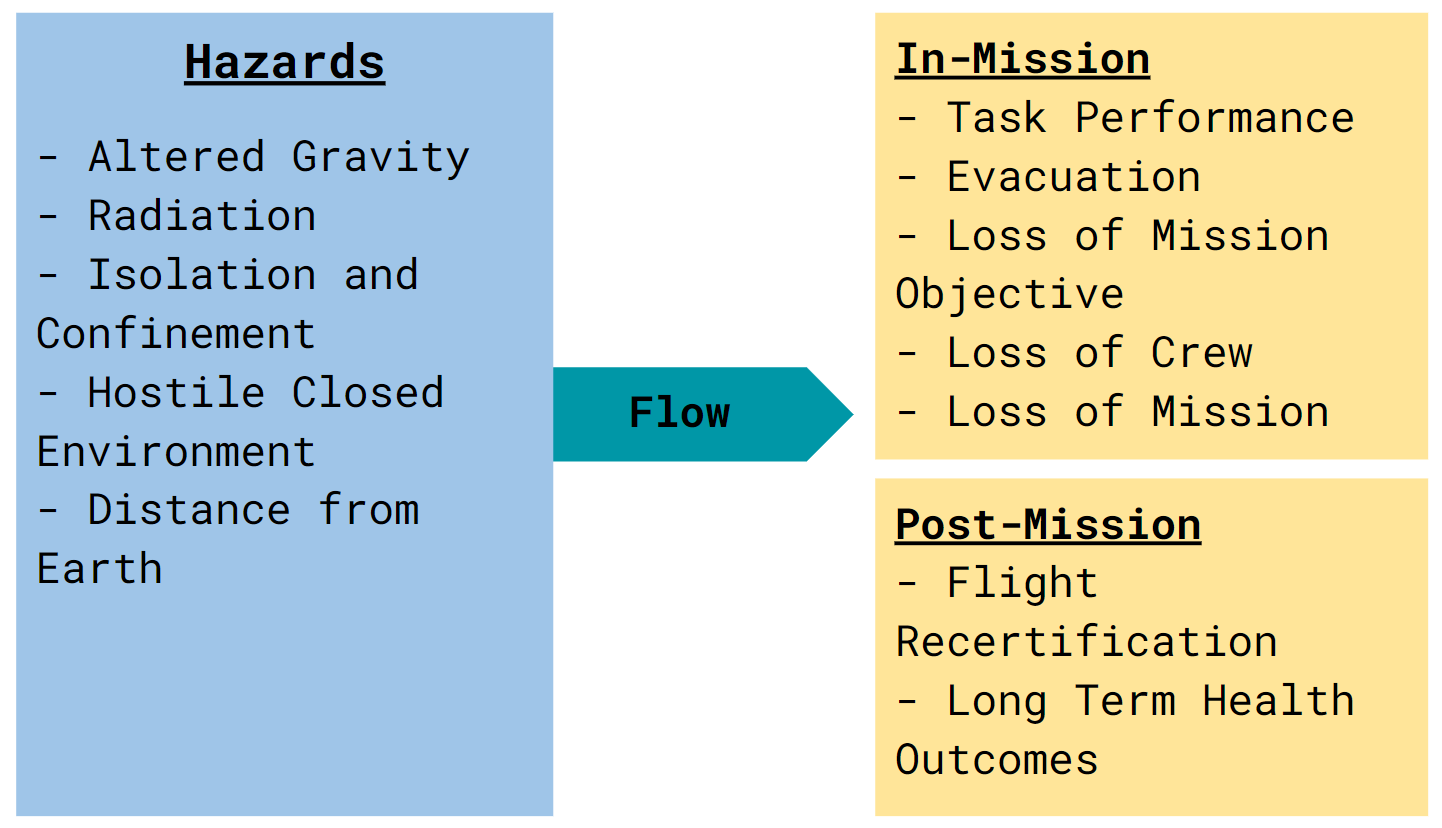
\includegraphics[width=\textwidth,height=\textheight,keepaspectratio]{flow.png}



\section{Theory}
\paragraph{Bayesian networks}
You can represent these relationships between variables by building a Bayesian networks.
Where it shows the representation of how nodes/variables interact with each other (direct dependencies between variables) → Allows the user to affirm and make accurate predictions based on observed data. 

For instance, if we observe that the weather is rainy, we can use the Bayesian network to estimate the probability of carrying an umbrella and the probability of the ground being wet. We can also do the reverse: if we know the ground is wet, we can estimate the probability that it is raining.
By using probabilities and the relationships encoded in the graph, Bayesian networks allow us to reason and make inferences about the variables even when we have incomplete or uncertain information.

\paragraph{Constraint-based methods (What IAMB Variations do)}
Discover the dependencies and relationships between nodes based on data by imposing certain constraints. Identify statistical dependencies between nodes → infer the underlying structure of the Bayesian network
\begin{itemize}
  \item Independence Testing: Determines the statistical independence or dependence between pairs of variables in the data. 
  Test whether the variables are conditionally independent given other variables. 
  If two variables are found to be independent, it suggests that there is no direct edge between them in the Bayesian network.
  
  \item Skeleton Discovery: Constructs a skeleton or an initial structure for the Bayesian network. 
  Represents the presence or absence of edges between variables. 
  Edges are added to the graph for variables that are found to be dependent, indicating a potential causal relationship.
   
  \item Orientation of Edges: Determine the orientation of the edges in the network.
  Establish the direction of causality between variables. 
  Examining conditional dependencies and using additional tests or heuristics to infer the most likely direction of causal influence.  
\end{itemize}

\paragraph{Markov Blanket}
The Markov blanket of a variable in a Bayesian network: Minimal set of variables that contains all the information necessary to predict the variable's value, given the values of other variables in the network.

Formally, the Markov blanket of a variable X in a Bayesian network consists of three sets of variables:
\begin{itemize}
  \item Parents of X: These are the variables that directly influence the value of X. If A is influenced by B, then B would be a parent of A.
  \item Children of X: These are the variables that are directly influenced by the value of X. If C is influenced by A, then C would be a child of A.
  \item Parents of X's children: These are the variables that are parents of X's children. If C is influenced by B, then B would be a parent of C's child (C) and would be included in the Markov blanket of A.
\end{itemize}

Simpler terms: Imagine you have three variables: Cloudy, Rain, Wet Grass. 
From what you know (observed data), they do influence each other's decisions. Rain's Markov blanket consists of the variables that directly influence it. It will form a special group that has all the information needed to understand how rain will happen.

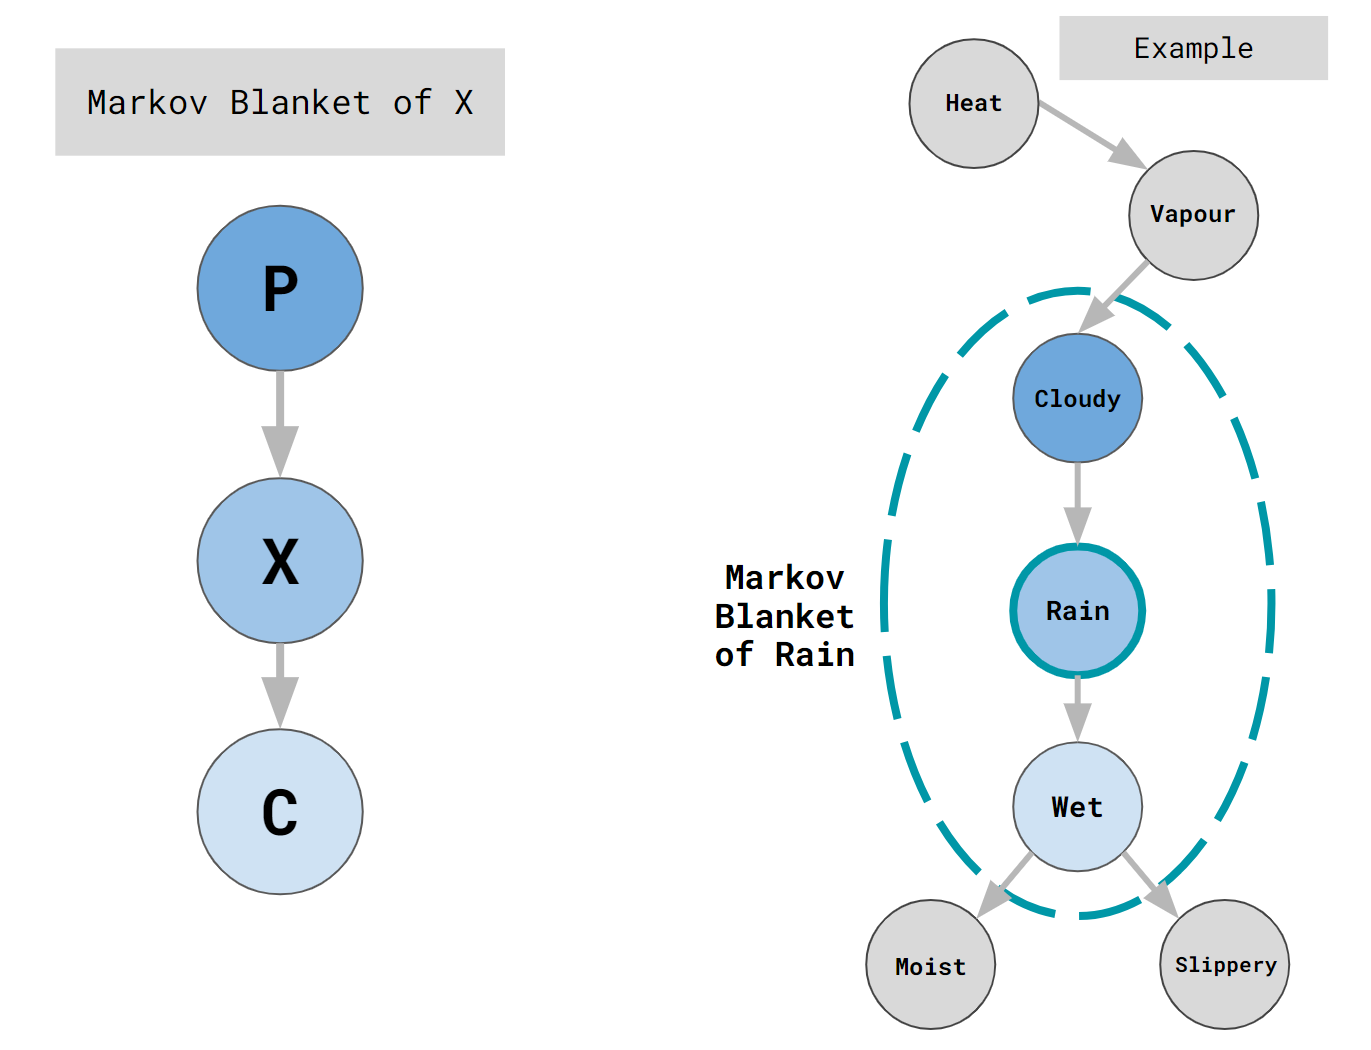
\includegraphics[width=\textwidth,height=\textheight,keepaspectratio]{mb.png}

So, who would be in Rain's Markov blanket? Firstly, it would include Cloudy because, from 21 years of living, you know if its cloudy -> High-chance it will rain! Secondly, it would include any nodes that are directly influenced by rain, like wet grass, wet floor, or cold.

If you think "Rain" as a person, Rain's Markov blanket is like a small group of people who are most important to her decision-making. If you know what these people are doing, you can make a pretty good guess about what Rain is likely to do.

In a Bayesian network, Markov blanket (MB) of a variable is the group of variables that have a direct influence on it or are directly influenced by it. It's the minimal set of variables that you need to pay attention to in order to understand and predict the behavior of that variable, without worrying about all the other variables in the network.

The Markov blanket concept helps us simplify things by focusing on a smaller, important group rather than considering the entire network. It allows us to make predictions or perform calculations about a specific variable by looking only at the variables in its Markov blanket.

Generally the process of finding the Markov blanket of a variable is called Markov blanket discovery. It is a key step in many algorithms for learning the structure of a Bayesian network from data. And its Pseudo-code is as follows:
\begin{lstlisting}
  # 1. Preprocess the data: Handle data cleaning, handling missing values
  data = preprocess_data(data)
  
  # 2. Define the set of variables and their relationships
  variables = get_variables_from_data(data)
  causal_relationships = define_causal_relationships()
  
  # 3. Initialize the Markov Blanket for each variable
  markov_blanket = {}
  for variable in variables:
      markov_blanket[variable] = find_markov_blanket(variable, data)
  
  # 4. Learn causal relationships from the Markov Blanket
  bayesian_network = create_empty_bayesian_network()
  for variable in variables:
      parents = find_parents(variable, markov_blanket[variable])
      for parent in parents:
          bayesian_network.add_edge(parent, variable)
  
  # 5. Output the Bayesian Network
  bayesian_network.to_graph()
  \end{lstlisting}


\section{Algorithm Description}

\subsection{IAMB | Incremental Association Markov Blanket}
Consists of two phases, a forward and a backward one. An estimate or copy of the Markov Blanket of a variable of interest $T$ is kept in the $MB$. 
In the forward phase all variables that belong in $MB(T)$, including false positives enter $CMB$ (Copy of MB) while in the backward phase the false positives are identified and removed so that $CMB = MB(T)$ in the end. 

Phase I is the following: start with an empty candidate set for the $CMB$ and admit into it (in the next iteration) the variable that maximizes a heuristic function  $f(X ; T | CMB)$. This is a measure of association between $X$ and $T$ given $CMB$. 
In backward conditioning (Phase II) we remove one-by-one the features that do not belong to the $MB(T)$ by testing whether a feature $X$ from $CMB$ is independent of $T$ given the remaining $CMB$.
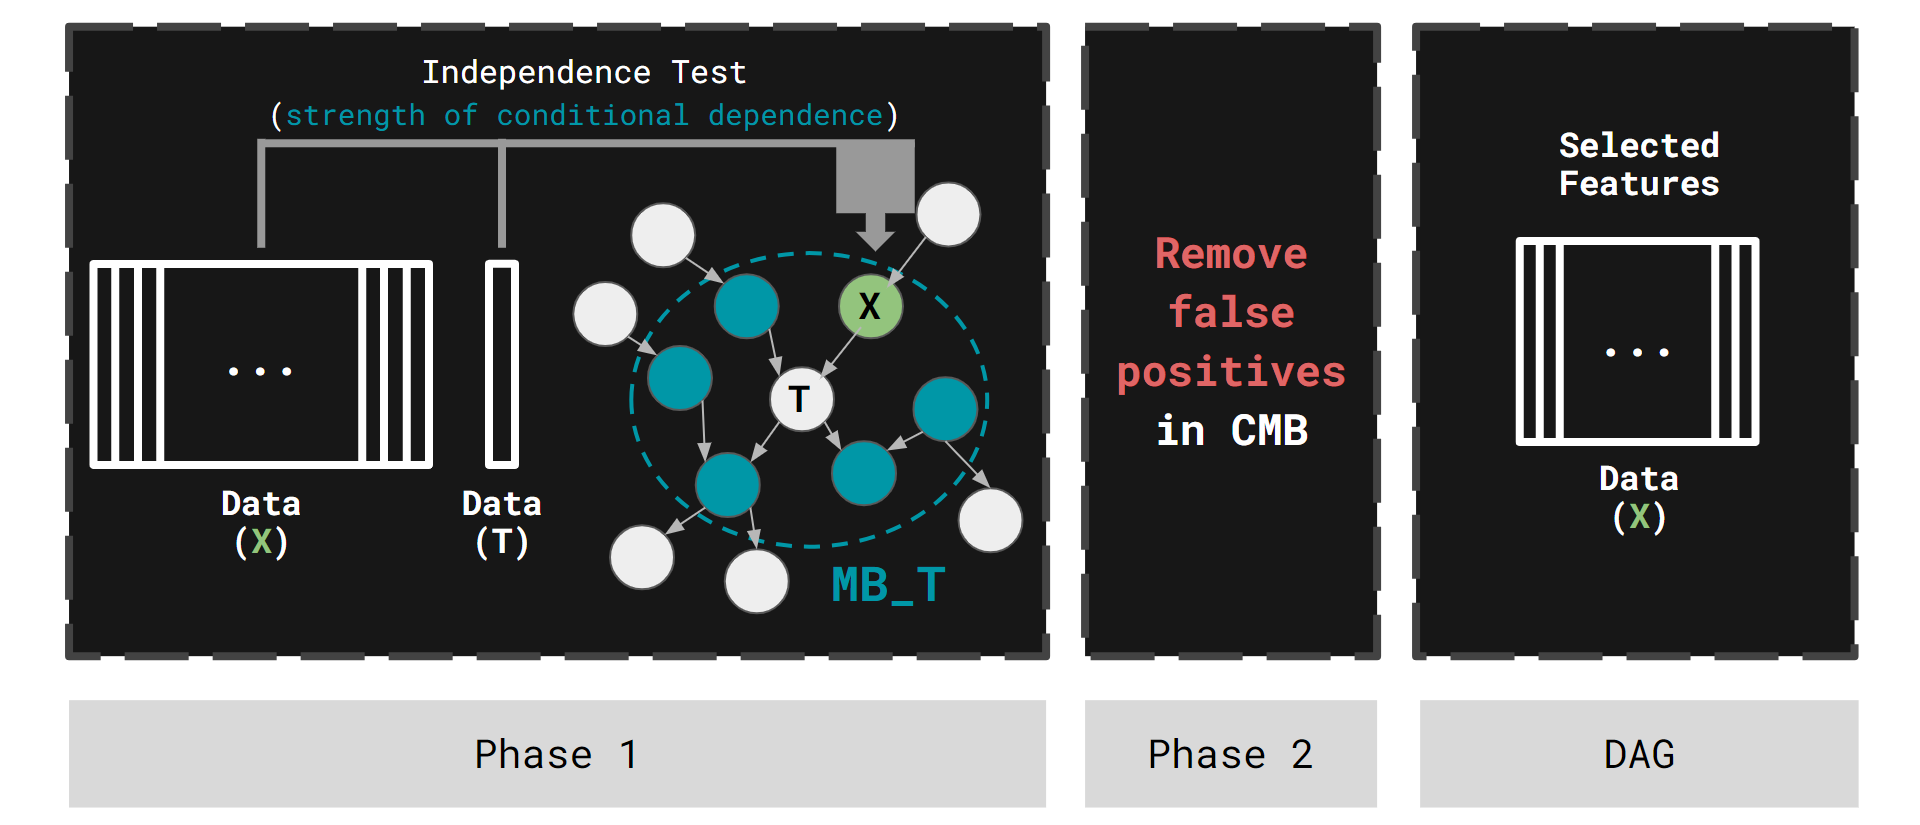
\includegraphics[width=\textwidth,height=\textheight,keepaspectratio]{iamb.png}


\subsection{Fast-IAMB | Fast-Incremental Association Markov Blanket}
Considered to be an improvement over the IAMB algorithm that aims to reduce the computational complexity.
It aims to reduce the computational and time complexity of the algorithm by pruning unnecessary tests.
Maintaining an order of the variables based on their likelihood of being in the Markov blanket.
Uses a combination of forward and backward steps to efficiently determine the Markov blanket for each variable.

Instead of relying on traditional statistical tests like chi-squared (kai-squared). 
It uses a combination of forward and backward steps to determine the $MB$ for each variable.
Computationally this is just $O(n)$ while IAMB is $O(2n)$ where it needs go forward and backward, here it does it in 1 loop.
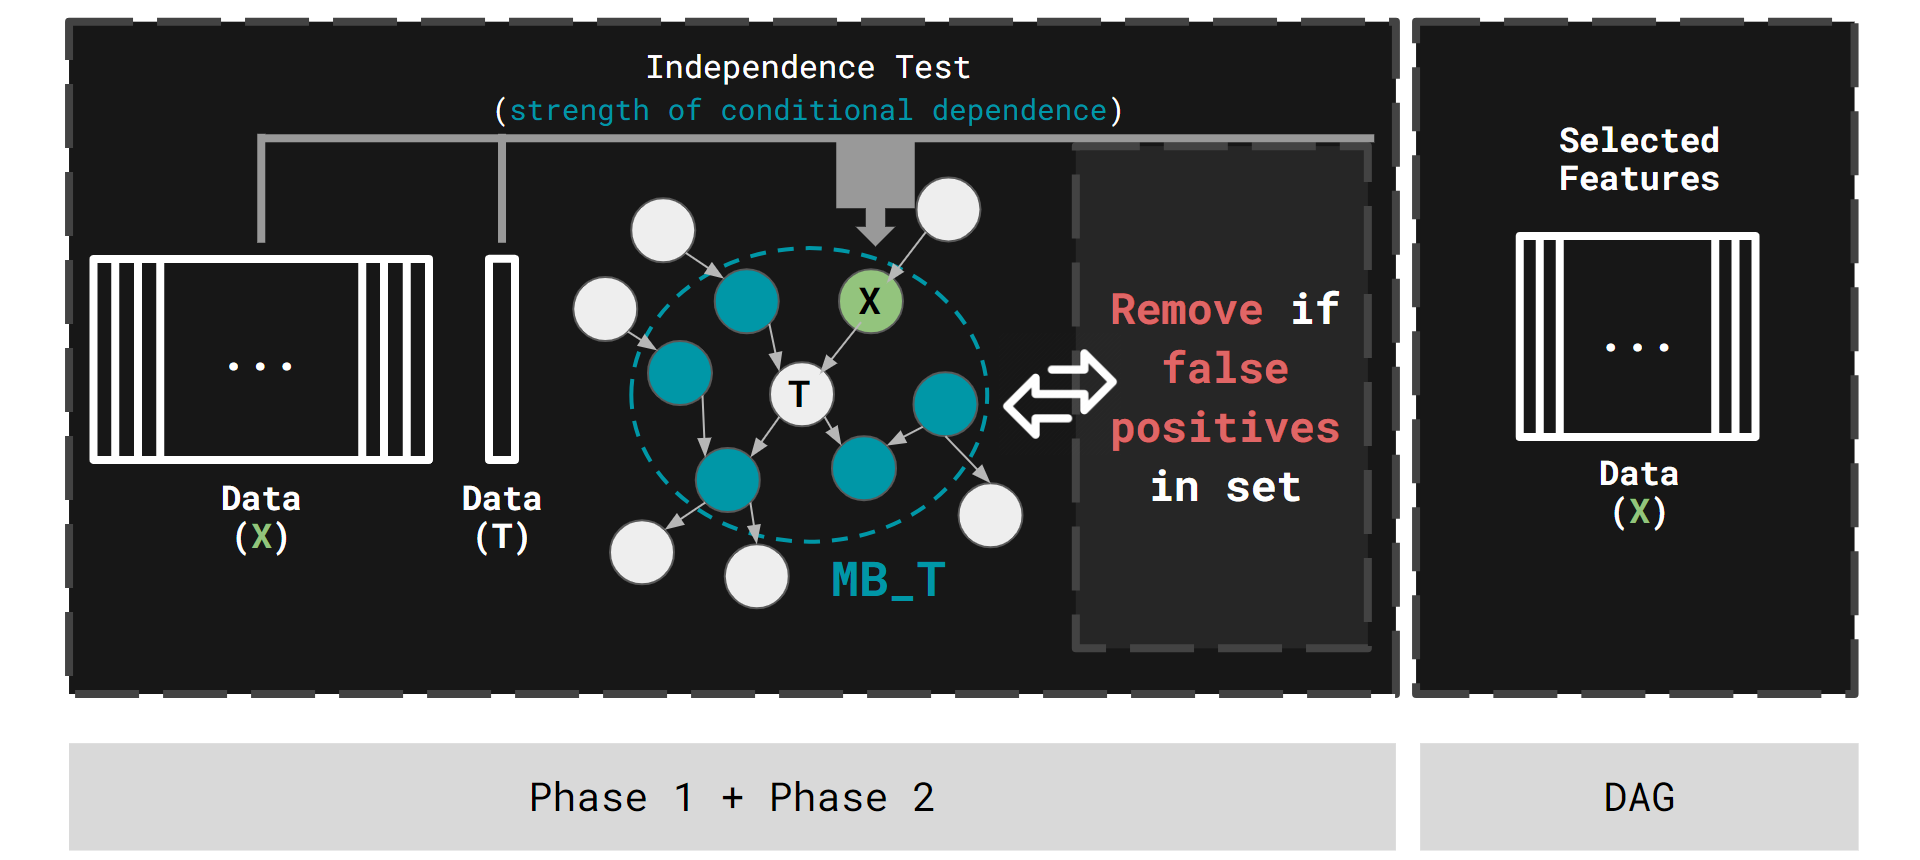
\includegraphics[width=\textwidth,height=\textheight,keepaspectratio]{fastiamb.png}


\subsection{Inter-IAMB | Interleaved Incremental Association Markov Blanket}
Extension of the IAMB algorithm that introduces an interleaved strategy for constructing the Markov blanket. 
Instead of iterating and processing one target variable at a time, it selects multiple target variables from the dataset and performs interleaved passes over the variables, gradually refining the Markov blankets. 
Allows for more efficient identification of variable dependencies and can lead to improved results in certain scenarios.

For each selected target variable $T$, it just perform the regular IAMB algorithm based on independence tests.
But after a short duration of processing, it switch to another target variable and continue the process. 
The switching between target variables is the "interleaving" part of the algorithm. 
By interleaving the runs, the algorithm can potentially reduce the total number of independence tests required and, thus, improve computational efficiency.
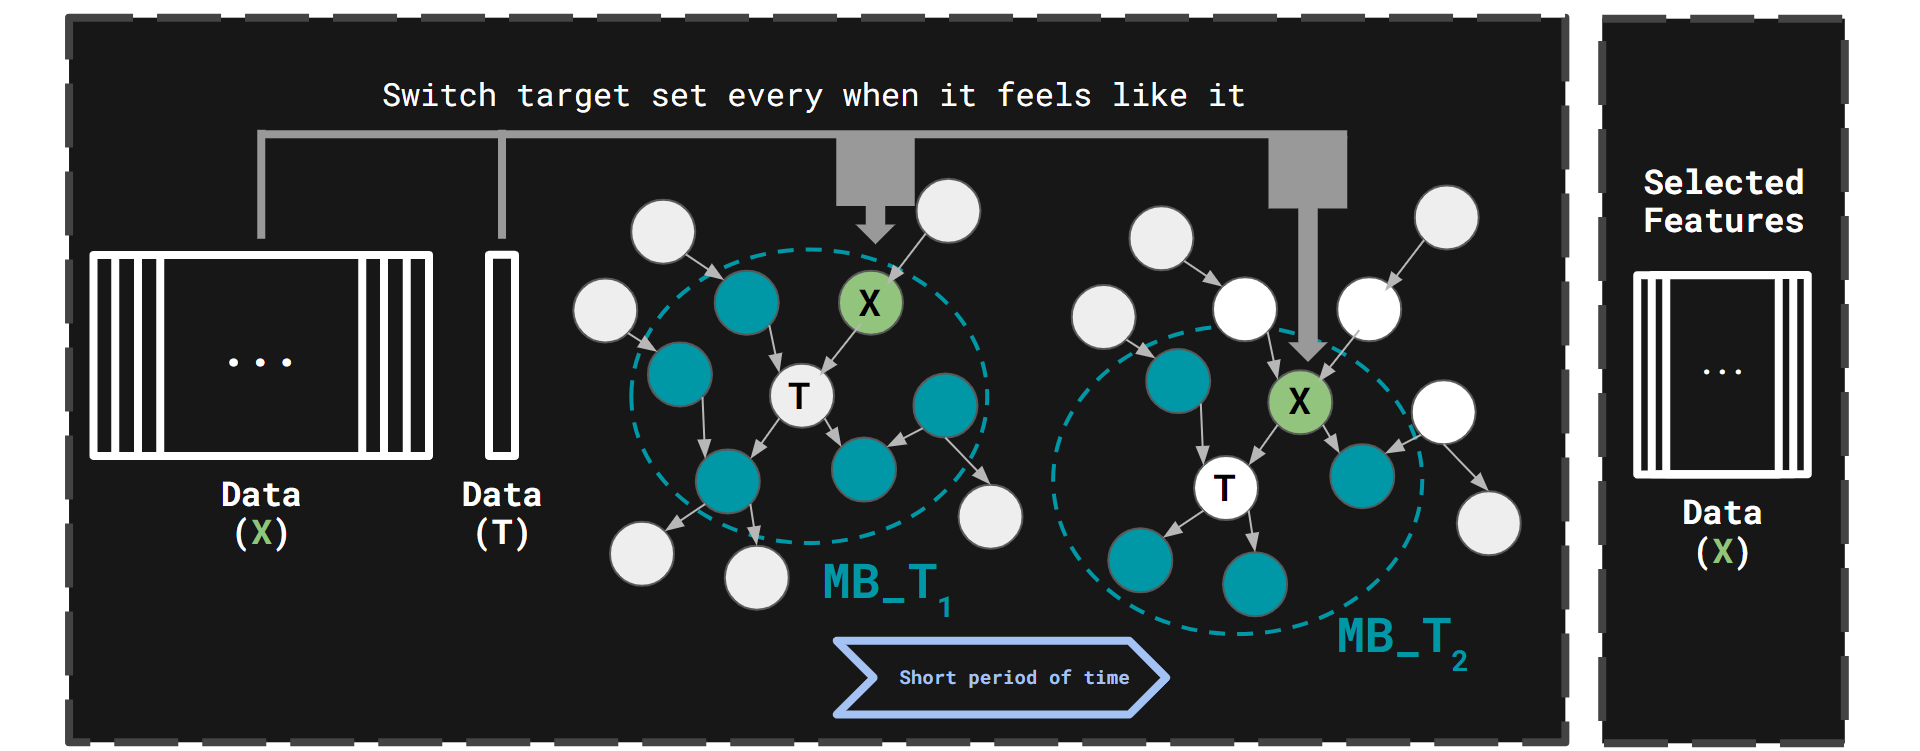
\includegraphics[width=\textwidth,height=\textheight,keepaspectratio]{interiamb.png}


\subsection{IAMB-FDR | Incremental Association Markov Blanket with False Discovery Rate Control}
Variant of the IAMB algorithm that incorporates false discovery rate (FDR) control to address the issue of multiple hypothesis testing. 
In structure learning, multiple statistical tests are performed, and without proper control, this can lead to an increased chance of false discoveries. 
IAMB-FDR applies FDR control techniques to adjust the statistical significance thresholds used in independence tests, thereby mitigating the risk of false discoveries and improving the reliability of the learned structure.
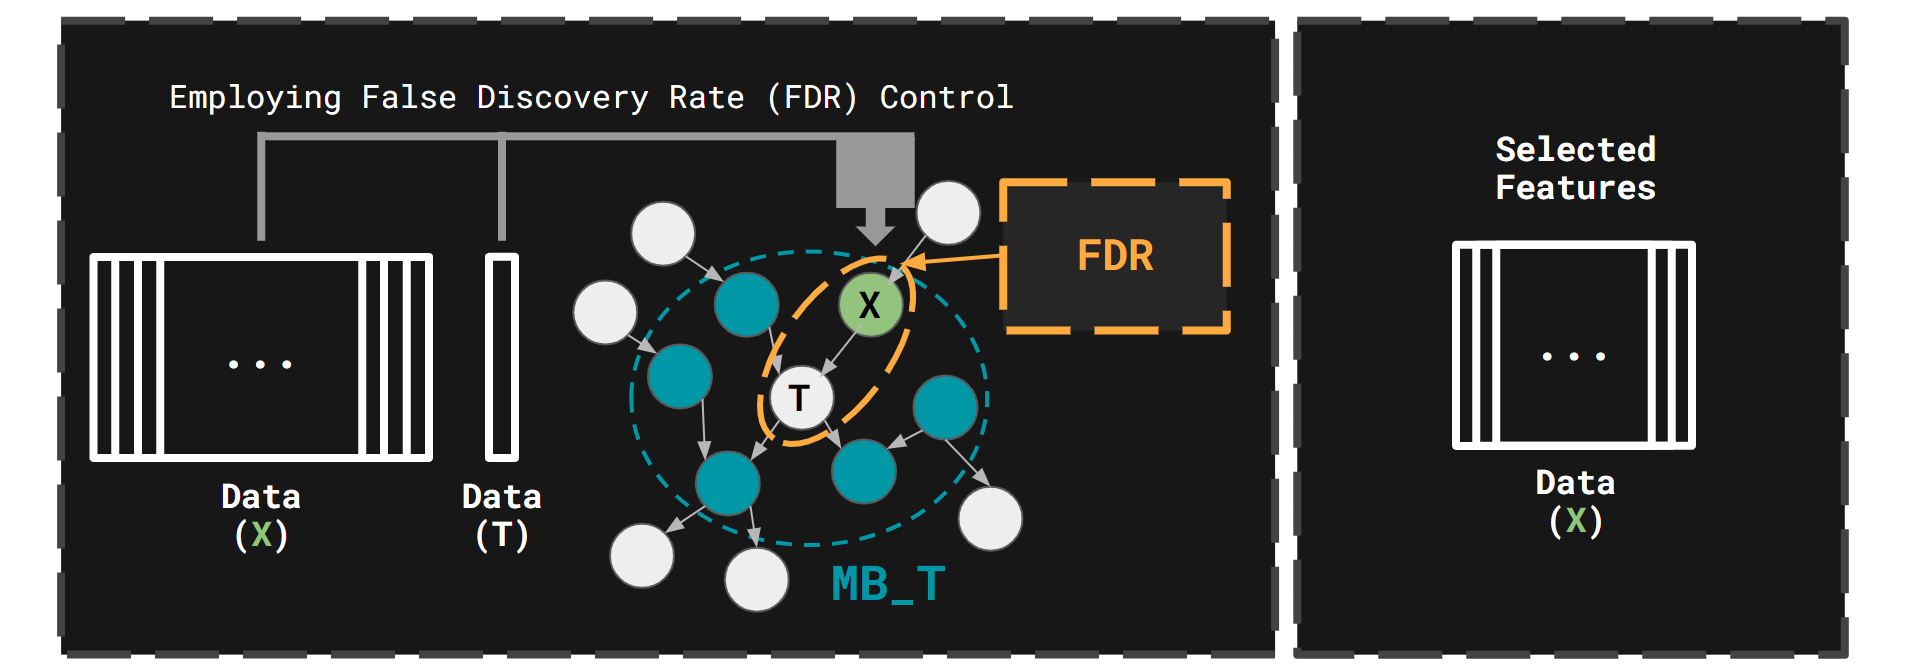
\includegraphics[width=\textwidth,height=\textheight,keepaspectratio]{iambfdr.png}




\section{Data Construction}


\section{Results and Outputs}


\section{Analysis and Discussion}


\section{Conclusion}



% \section{Examples of citations, figures, tables, references}
% \label{sec:others}
% \lipsum[8] \cite{kour2014real,kour2014fast} and see \cite{hadash2018estimate}.

% The documentation for \verb+natbib+ may be found at
% \begin{center}
%   \url{http://mirrors.ctan.org/macros/latex/contrib/natbib/natnotes.pdf}
% \end{center}
% Of note is the command \verb+\citet+, which produces citations
% appropriate for use in inline text.  For example,
% \begin{verbatim}
%    \citet{hasselmo} investigated\dots
% \end{verbatim}
% produces
% \begin{quote}
%   Hasselmo, et al.\ (1995) investigated\dots
% \end{quote}

% \begin{center}
%   \url{https://www.ctan.org/pkg/booktabs}
% \end{center}


% \subsection{Figures}
% \lipsum[10] 
% \footnote{Sample of the first footnote.}
% \lipsum[11] 

% \begin{figure}
%   \centering
%   \fbox{\rule[-.5cm]{4cm}{4cm} \rule[-.5cm]{4cm}{0cm}}
%   \caption{Sample figure caption.}
%   \label{fig:fig1}
% \end{figure}

% \begin{equation}
%   \xi _{ij}(t)=P(x_{t}=i,x_{t+1}=j|y,v,w;\theta)= {\frac {\alpha _{i}(t)a^{w_t}_{ij}\beta _{j}(t+1)b^{v_{t+1}}_{j}(y_{t+1})}{\sum _{i=1}^{N} \sum _{j=1}^{N} \alpha _{i}(t)a^{w_t}_{ij}\beta _{j}(t+1)b^{v_{t+1}}_{j}(y_{t+1})}}
% \end{equation}

% \subsection{Tables}
% \lipsum[12]
% See awesome Table~\ref{tab:table}.

% \begin{table}
%  \caption{Sample table title}
%   \centering
%   \begin{tabular}{lll}
%     \toprule
%     \multicolumn{2}{c}{Part}                   \\
%     \cmidrule(r){1-2}
%     Name     & Description     & Size ($\mu$m) \\
%     \midrule
%     Dendrite & Input terminal  & $\sim$100     \\
%     Axon     & Output terminal & $\sim$10      \\
%     Soma     & Cell body       & up to $10^6$  \\
%     \bottomrule
%   \end{tabular}
%   \label{tab:table}
% \end{table}

% \subsection{Lists}
% \begin{itemize}
% \item Lorem ipsum dolor sit amet
% \item consectetur adipiscing elit. 
% \item Aliquam dignissim blandit est, in dictum tortor gravida eget. In ac rutrum magna.
% \end{itemize}


\bibliographystyle{unsrt}  
% \bibliography{references}  %%% Remove comment to use the external .bib file (using bibtex).
%% and comment out the ``thebibliography'' section.


%%% Comment out this section when you \bibliography{references} is enabled.
\begin{thebibliography}{1}


\bibitem{}
Antonsen, Erik L., et al.
\newblock Directed Acyclic Graphs: A Tool for Understanding the NASA Human Spaceflight System Risks - Human System Risk Board.
\newblock In {\em NTRS - NASA Technical Reports Server, 1 Oct. 2022}, ntrs.nasa.gov/citations/20220015709.

\bibitem{}
Erik L.
\newblock Human System Risk Management Plan.
\newblock In {\em NTRS - NASA Technical Reports Server, 1 Oct. 2022}, https://ntrs.nasa.gov/citations/20205008887.

\bibitem{}
Erik L., Robert J., et al.
\newblock Directed Acyclic Graph Guidance Documentation.
\newblock In {\em NTRS - NASA Technical Reports Server, 1 Jun. 2022}, https://ntrs.nasa.gov/citations/20220006812.

\bibitem{}
Robert J., Ryan T., et al.
\newblock Validating Causal Diagrams of Human Health Risks for Spaceflight: An Example Using Bone Data from Rodents.
\newblock In {\em National Library of Medicine, 5 Sep. 2022}, https://pubmed.ncbi.nlm.nih.gov/36140288/.

\bibitem{}
Philipp M., Leena C., et al.
\newblock Self-Compatibility: Evaluating Causal Discovery without Ground Truth.
\newblock In {\em NTRS - NASA Technical Reports Server, 18 Jul. 2023}, https://arxiv.org/abs/2307.09552.


\end{thebibliography}


\end{document}
